\section{Running EnergyPlus, Building Envelope, Internal Loads, Reports}\label{running-energyplus-building-envelope-internal-loads-reports}

\subsection{Overview}\label{overview}

\begin{itemize}
\item
  Rectangular single story building
\item
  Windows in east and west walls
\item
  Single zone with no interior partitions
\item
  Lightweight construction
\end{itemize}

\begin{figure}[hbtp] % fig 11
\centering
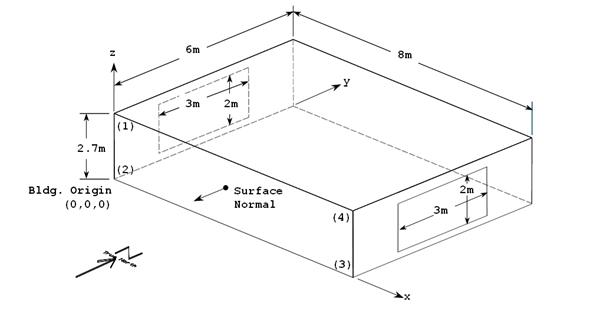
\includegraphics[width=0.9\textwidth, height=0.9\textheight, keepaspectratio=true]{media/image011.jpg}
\caption{Schematic for Exercise 1 \protect \label{fig:schematic-for-exercise-1}}
\end{figure}

The details of the building construction and operation are shown in the following tables and description. For tutorial purposes, the building is located in Chicago Illinois, one of the weather files supplied with EnergyPlus. These details are listed in a fashion to make for easy entry into EnergyPlus.

\subsection{Details of the exercise}\label{details-of-the-exercise}

\subsubsection{Surface Constructions}\label{surface-constructions}

\begin{longtable}[c]{p{1.5in}p{4.5in}}
\caption{Additional Model Details \label{table:additional-model-details}} \tabularnewline
\toprule 
Type & Details \tabularnewline
\midrule
\endfirsthead

\caption[]{Additional Model Details} \tabularnewline
\toprule 
Type & Details \tabularnewline
\midrule
\endhead

Internal Loads & Lights (1000 W), Office Lighting schedule, surface mount fluorescent \tabularnewline
Space Conditioning & Heating setpoint 20C, cooling setpoint 24C, no setback \tabularnewline
Location & Chicago, Illinois, USA; Summer and Winter design days \tabularnewline
Simulation Period & Annual, Jan 1 - Dec 31 \tabularnewline
Ground Temperatures & 18.2 C to 22.5 C (from Slab preprocessor, vary monthly) \tabularnewline
\bottomrule
\end{longtable}

\subsubsection{Window Properties}\label{window-properties}

\begin{longtable}[c]{p{1.5in}p{4.5in}}
\caption{Additional Model Details \label{table:additional-model-details}} \tabularnewline
\toprule 
Type & Details \tabularnewline
\midrule
\endfirsthead

\caption[]{Additional Model Details} \tabularnewline
\toprule 
Type & Details \tabularnewline
\midrule
\endhead

Internal Loads & Lights (1000 W), Office Lighting schedule, surface mount fluorescent \tabularnewline
Space Conditioning & Heating setpoint 20C, cooling setpoint 24C, no setback \tabularnewline
Location & Chicago, Illinois, USA; Summer and Winter design days \tabularnewline
Simulation Period & Annual, Jan 1 - Dec 31 \tabularnewline
Ground Temperatures & 18.2 C to 22.5 C (from Slab preprocessor, vary monthly) \tabularnewline
\bottomrule
\end{longtable}

Refers to specific glass type included in the EnergyPlus datasets directory

~(\textbf{WindowGlassMaterials.idf})

\begin{longtable}[c]{p{1.5in}p{4.5in}}
\caption{Additional Model Details \label{table:additional-model-details}} \tabularnewline
\toprule 
Type & Details \tabularnewline
\midrule
\endfirsthead

\caption[]{Additional Model Details} \tabularnewline
\toprule 
Type & Details \tabularnewline
\midrule
\endhead

Internal Loads & Lights (1000 W), Office Lighting schedule, surface mount fluorescent \tabularnewline
Space Conditioning & Heating setpoint 20C, cooling setpoint 24C, no setback \tabularnewline
Location & Chicago, Illinois, USA; Summer and Winter design days \tabularnewline
Simulation Period & Annual, Jan 1 - Dec 31 \tabularnewline
Ground Temperatures & 18.2 C to 22.5 C (from Slab preprocessor, vary monthly) \tabularnewline
\bottomrule
\end{longtable}
